\documentclass[a4paper]{article}

\usepackage[intlimits]{amsmath}
\usepackage{mathrsfs}
\usepackage{amsthm}
\usepackage{amssymb}
\usepackage{cancel}
\usepackage{graphicx}
\usepackage{color}
\usepackage{natbib}
\usepackage{hyperref}
\usepackage{listings}
\usepackage{parskip}
\usepackage[margin=1.3in]{geometry}
\usepackage{abstract}
\usepackage{multicol}
\usepackage{float}

\citestyle{apalike}
\bibliographystyle{apalike}

\providecommand{\e}[1]{\times10^{#1}}
\providecommand{\units}[1]{\;\mathrm{#1}}
\providecommand{\data}[2]{$#1\units{#2}$}
\providecommand{\diff}[2]{\frac{\partial #1}{\partial #2}}
\providecommand{\ddiff}[2]{\frac{\partial^2 #1}{\partial #2^2}}
\providecommand{\tdiff}[2]{\frac{\mathrm{d} #1}{\mathrm{d} #2}}
\providecommand{\infint}[2]{\int\limits_{-\infty}^{\infty}{#1}\;\mathrm{d}#2}
\providecommand{\dd}{\;\mathrm{d}}
\providecommand{\MAA}{\text{\AA}}
\providecommand{\abs}[1]{\left| #1 \right|} % for absolute value
\providecommand{\avg}[1]{\left< #1 \right>} % for average
\providecommand{\grad}[1]{\gv{\nabla} #1} % for gradient
\providecommand{\bigo}[1]{\mathcal{O}\left( #1 \right)}

\let\divsymb=\div
\renewcommand{\div}[1]{\gv{\nabla} \cdot #1} % for divergence
\providecommand{\curl}[1]{\gv{\nabla} \times #1} % for curl
\providecommand{\MAA}{\text{\AA}}
\providecommand{\figwidth}{.45\columnwidth}
\newcommand\numberthis{\addtocounter{equation}{1}\tag{\theequation}}
\numberwithin{equation}{section}

\renewcommand{\bibname}{References}

\title{{A study of the characteristics of HiRes output on Herschel SPIRE Observations}}
\author{Tom Badran}

\date{July to September 2015}

\begin{document}

\maketitle

\section{Introduction}

This work is a continuation of the work in my final year undergraduate project \cite{badran} in order to establish a set of criteria for deciding whether HiRes should be applied in the SPIRE data processing pipeline, and sensible values for some of the parameters. This paper is recommended reading in order to study the techniques used for analyzing the image fidelity improvement achieved through HiRes.

\section{HiRes time Complexity}

\begin{figure}[H]
    \centering
    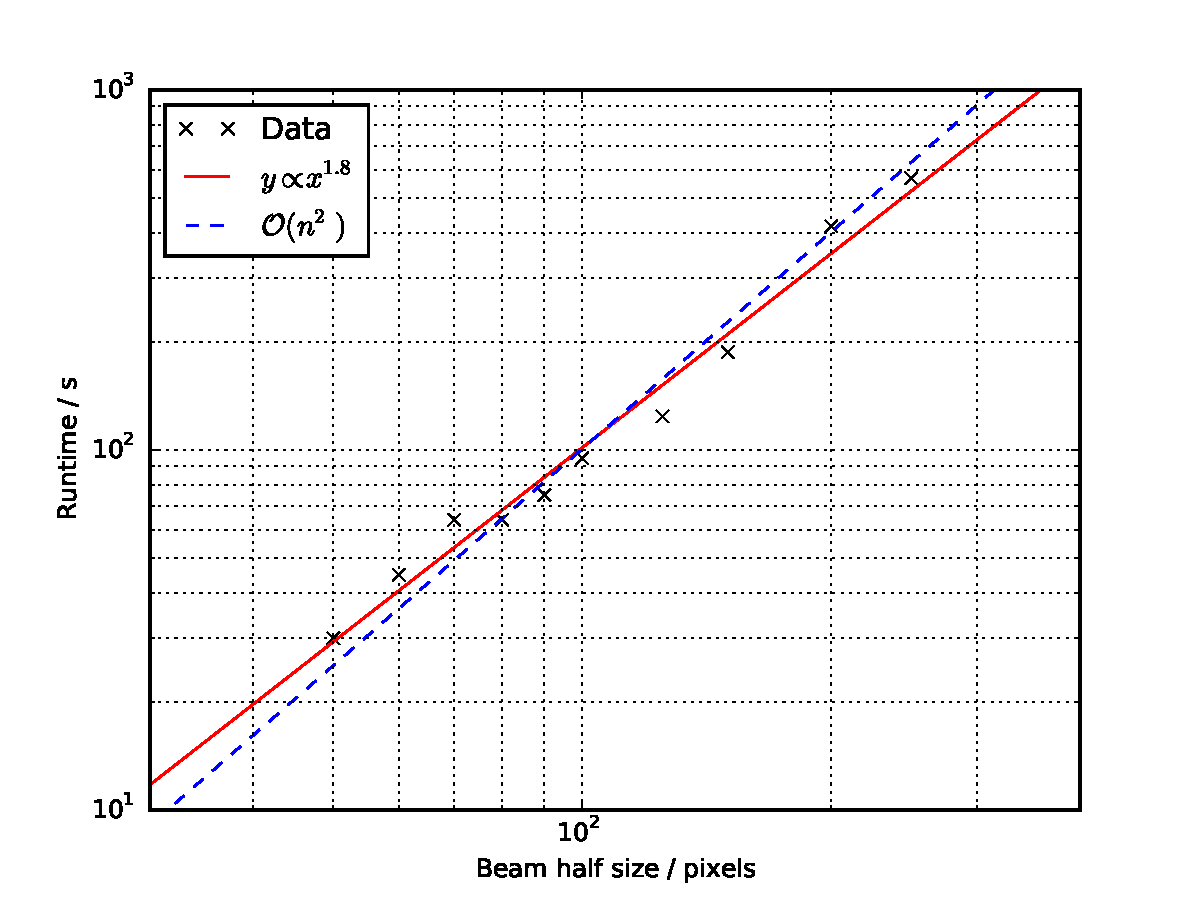
\includegraphics[width=0.85\linewidth]{runtime.pdf}
    \caption{Measurements of HiRes runtime as a function of the input beam half-width pixel size}
    \label{hrtc}
\end{figure}

To measure the time complexity of HiRes, it was run with a set of beams cropped to have specific beam half-widths. These runs were timed and the results shown in figure \ref{hrtc} were obtained.

Clearly HiRes has a runtime complexity of approximately $\bigo{n^{1.8}}$, so runs in approximately quadratic time (as would be expected for convolution) as a function of beam width. Clearly for the shorter wavelength observations we want to be able to minimize this beam size as much as possible in order to be able to perform HiRes on as much of the data as possible in a reasonable time.

\section{Adapting the Image Difference method}

The image differencing method used in \citep{badran} relied on manually placing an aperture over the region of interest in the observation, however it would be preferred to use the entire image where possible. However one of the properties of HiRes is that it flattens the background of the image down to zero, so if an observation contains a lot of background data with a region of interest in the center, we don't want this background flooring to skew the difference results.

In order to do this I created a weighting map based on proximity to bright pixels. This was done by applying a box blur to the truth image with a solid disc kernel, then dividing this map by the maximum value. This creates a weighting map where regions near to bright pixels will have a larger weight than the background.


\section{Fidelity of HiRes output as a function of input beam size}

To help make a decision on what beam size to use, we need to have an understanding of not just the time complexity, but also how the beam size affects the fidelity of the output from HiRes.

\begin{figure}[H]
    \centering
    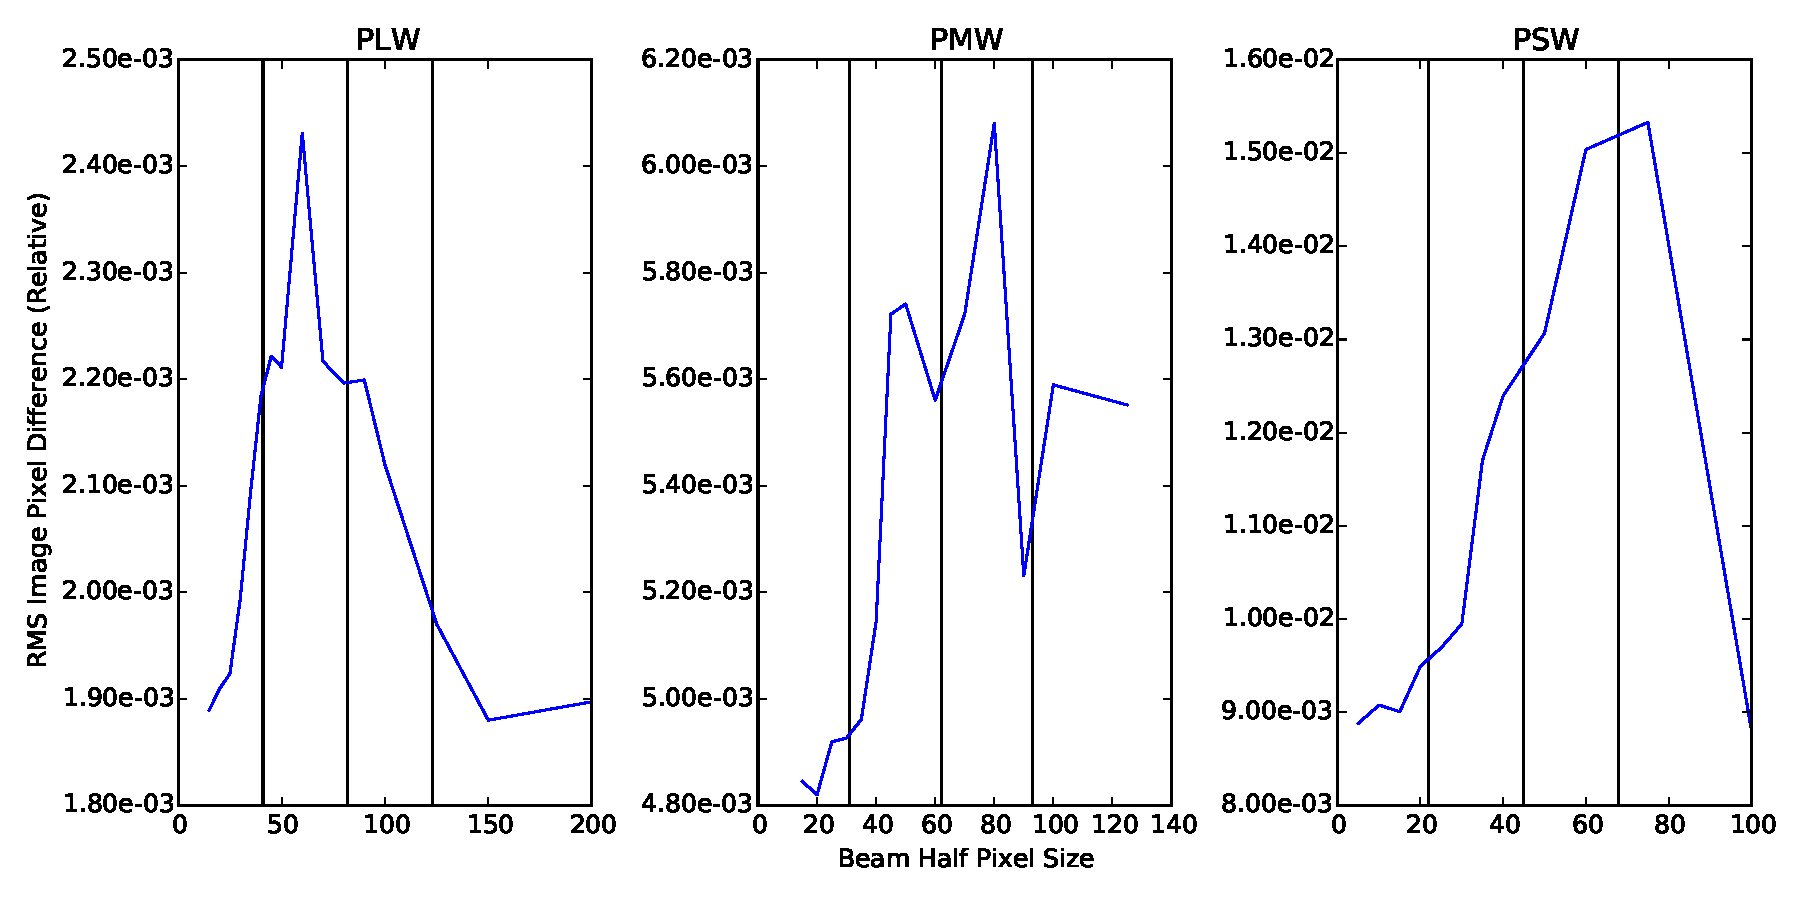
\includegraphics[width=0.85\linewidth]{beam-size-1342189427.pdf}
    \caption{M74 - Comparison of HiRes output to theoretical truth image, as a function of the input beam half-width pixel size. Vertical lines show locations of the first 3 beam minima}
    \label{beamsize-m74}
\end{figure}

\begin{figure}[H]
    \centering
    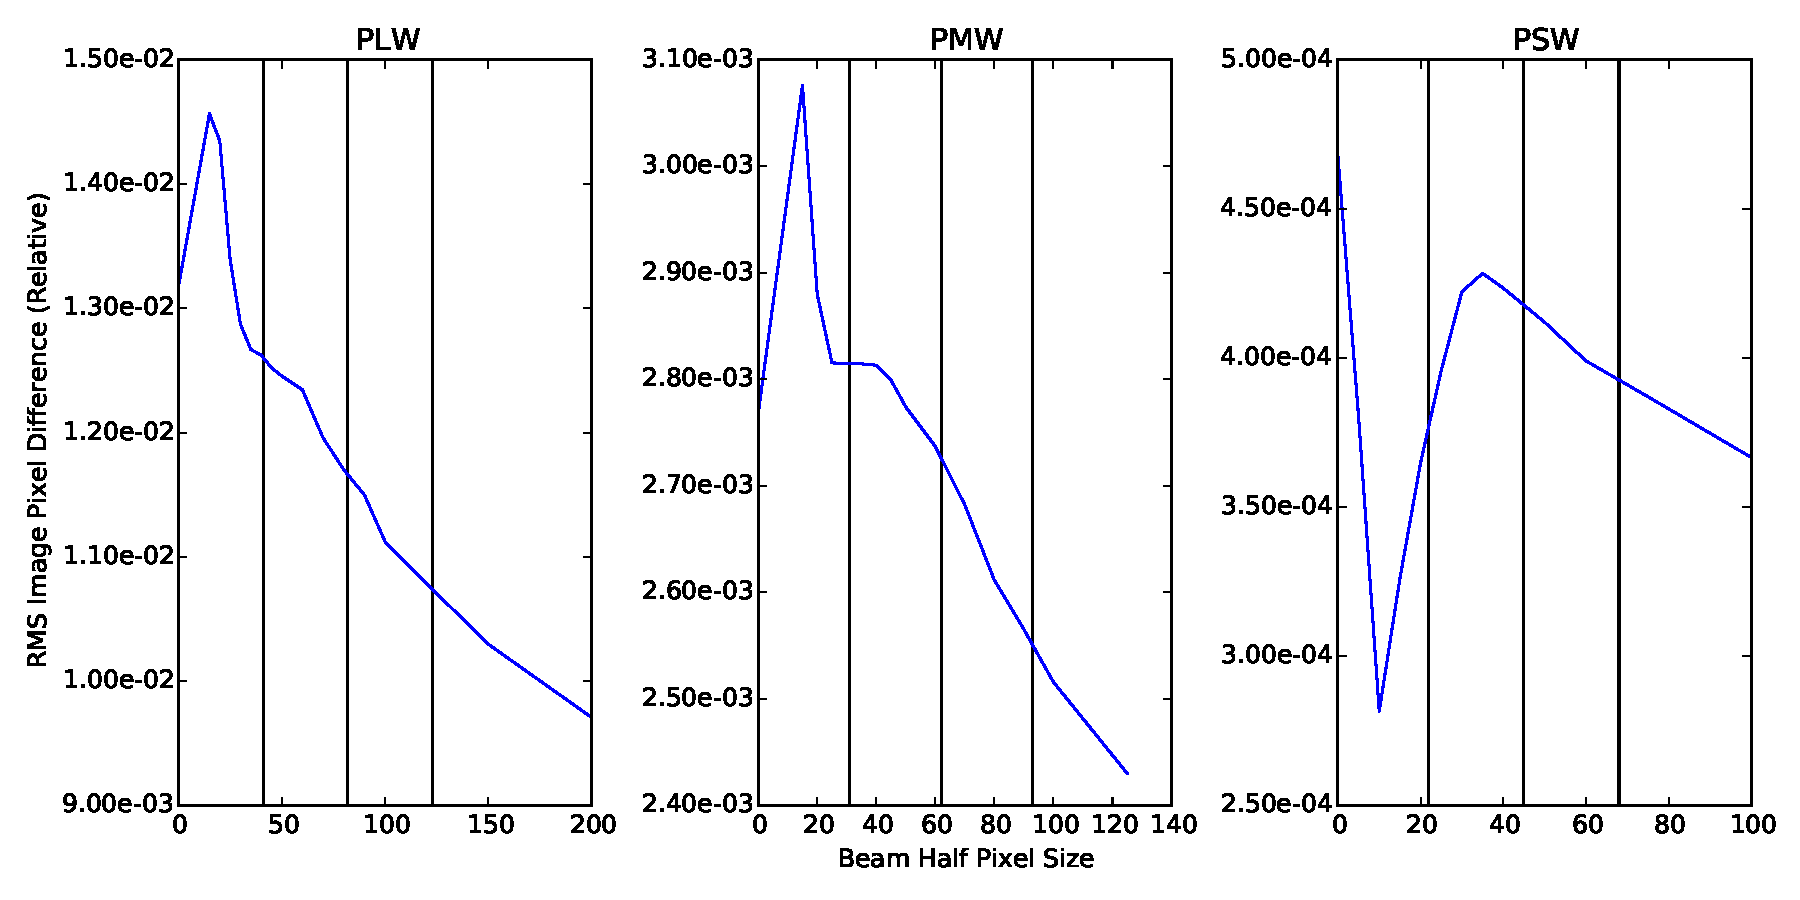
\includegraphics[width=0.85\linewidth]{beam-size-1342188588.pdf}
    \caption{NGC 4151 - Comparison of HiRes output to theoretical truth image, as a function of the input beam half-width pixel size. Vertical lines show locations of the first 3 beam minima}
    \label{beamsize-ngc4151}
\end{figure}

\begin{figure}[H]
    \centering
    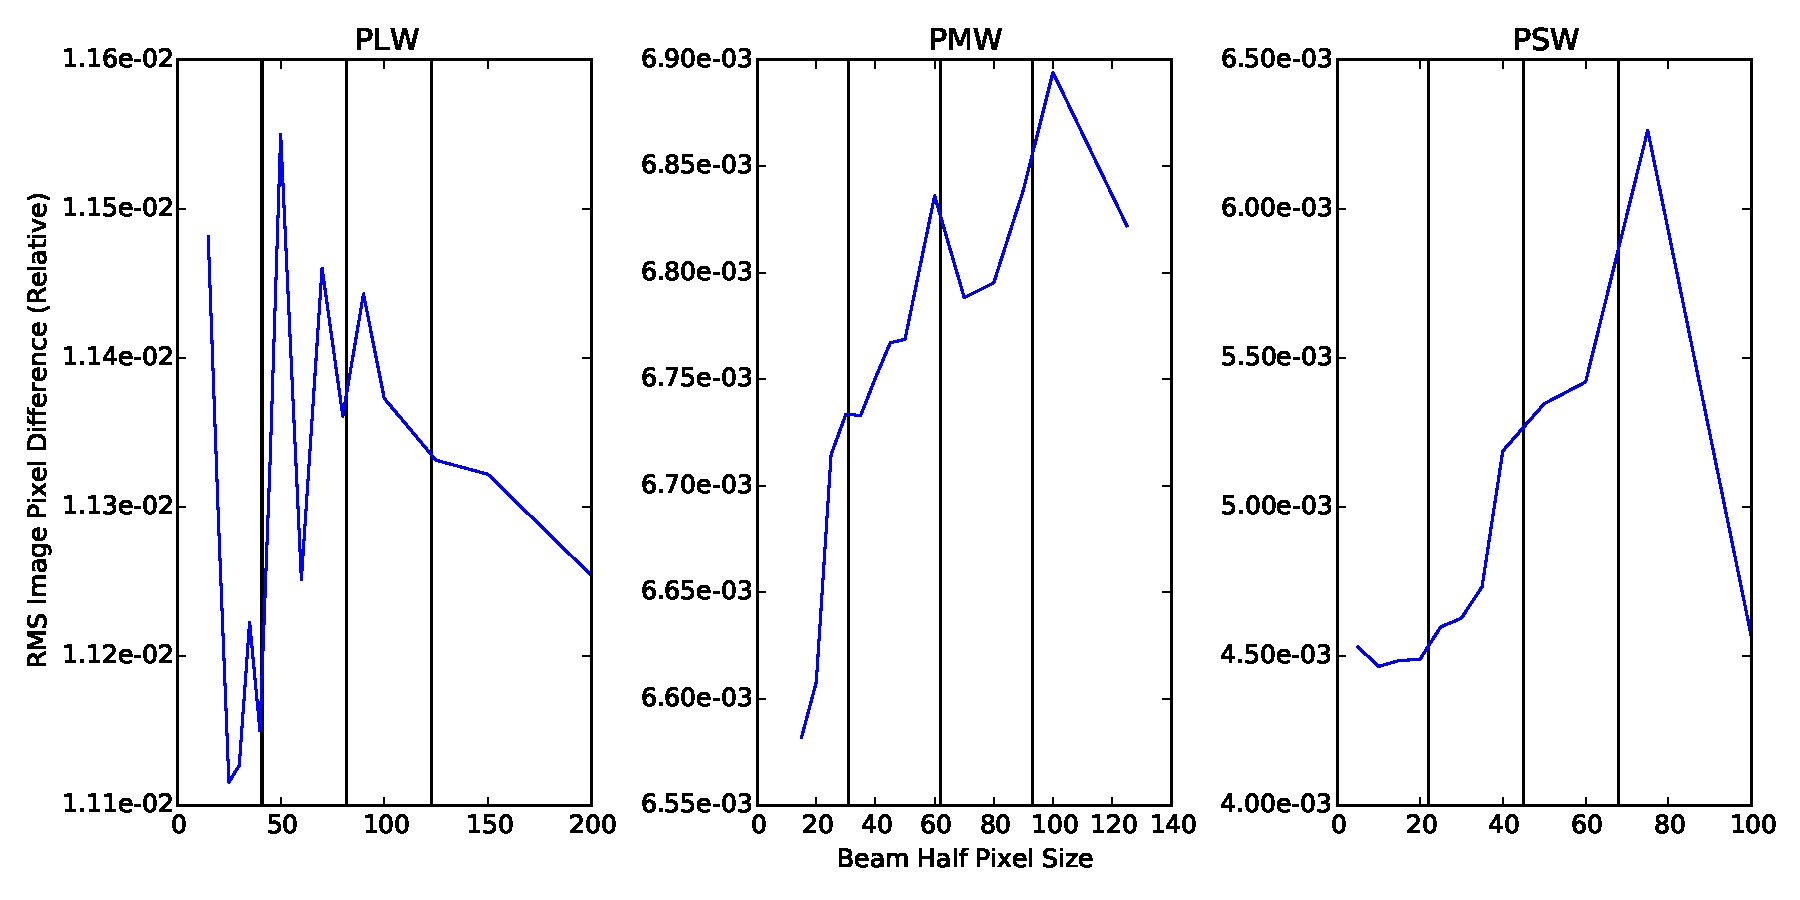
\includegraphics[width=0.85\linewidth]{beam-size-1342185538.pdf}
    \caption{M81 - Comparison of HiRes output to theoretical truth image, as a function of the input beam half-width pixel size. Vertical lines show locations of the first 3 beam minima}
    \label{beamsize-m81}
\end{figure}

Clearly shown in figures \ref{beamsize-m74}, \ref{beamsize-ngc4151} and \ref{beamsize-m81} there is an obvious improvement to the output of HiRes as the beam size increase, and it does appear that going to the 3'rd minima still has measurable benefits. The results for PSW are not so clear.

\section{Fidelity of HiRes output as a function of iterations}

\section{Recomendations}

\subsection{Beam Size}

It is recommended to set the beam size to include all the beam up to third minima.

For PLW and PMW it is recommended to set the default HiRes beam size to be at the third minima, or approximately 125 and 100 pixels wide respectively. Note that this is higher than the current default in the pipeline so may need to be adjusted due to considerations of computational time available.

\bibliography{references}

\end{document}
